

In this section, we examine the performance of ReLOOP using simulation. In particular, we consider how ReLOOP performs when varying sample size, the predictive power of the covariates, and the predictive power of the external predictions. Consider a randomized experiment in which there are $N$ subjects. The potential outcomes and covariates are generated from the following linear model:
\begin{align*}
a_i &= 2Z_{1,i} + Z_{2,i} + \delta_i \\
c_i &= \frac{ a_i }{ \sigma_{a} } \\
t_i &= c_i + 3
\end{align*}
where $\delta_i \sim \text{N}(0,\sigma_{gen}^2)$, $Z_{ij} \sim \text{Unif}(0,10)$, and $\sigma^2_{a} = \text{Var}(a_i) = \frac{500}{12} + \sigma_{gen}^2$. By generating our potential outcomes as above, we have defined our generative model such that the control potential outcomes have unit variance. We can alternatively write the observed outcome as:
\begin{align*}
Y_i &= 3 T_i + \frac{2}{\sigma_{a}}Z_{1,i} + \frac{1}{\sigma_{a}} Z_{2,i} + \epsilon_i
\end{align*}
where $\epsilon_i \sim \text{N}(0,\sigma_{gen}^2/\sigma^2_{a})$.
\\\\
For each observation, we also simulate external predictions $\tilde{t}_i$ and $\tilde{c}_i$ for $t_i$ and $c_i$ by taking the true $t_i$ or $c_i$ and adding a normally distributed noise term with mean 0 and standard deviation $\sigma_{ext}$.
\\\\
To reiterate, we wish to consider variations in sample size, the predictive power of the covariates, and the predictive power of the external predictions. Sample size is directly indexed with $N$. We can index the predictive power of the covariates using the control-side $R^2$:
\[ R_c^2 = 1 - \frac{ \sigma^2_{gen} }{ \sigma^2_{a} }. \]
Similarly, the predictive power of our external prediction $\tilde{c}_i$ is
\[ R^2_{p} = 1 - \frac{\sigma_{ext}^2}{\text{Var}( \tilde{c}_i )} = 1 - \frac{\sigma^2_{ext}}{1+\sigma^2_{ext}}. \]
Given a desired $R_c^2$ and $R^2_{p}$, we can calculate the corresponding values of $\sigma^2_{gen}$ and $\sigma^2_{ext}$ (note that $\sigma_{ext}^2$ and $\sigma_{gen}^2$ characterize the distribution of the external predictions and potential outcomes for a given set of covariates):
\begin{align*}
\sigma^2_{gen} &= \frac{1-R_c^2}{R_c^2}\times\frac{500}{12} \\
\sigma^2_{ext} &= \frac{1 - R^2_{p}}{R_p^2} .
\end{align*}
We perform three sets of simulations, in which we hold two of $N$, $R_c^2$, and $R^2_{p}$ constant and vary the third.  For each set of simulations, we compare the following methods:
\begin{enumerate}
	\item LOOP: uses the LOOP estimator including only the covariates $Z_1$ and $Z_2$
	\item LOOP with External Predictions: uses the LOOP estimator with external predictions as a covariate (in addition to $Z_1$ and $Z_2$)
	\item ReLOOP*: uses the LOOP estimator, with OLS as the imputation method. Only includes the external predictions as a covariate
	\item ReLOOP: interpolates between the previous two methods
\end{enumerate}
\noindent
We use the following simulation procedure. For a given set of $N$, $R_c^2$, and $R^2_{p}$, we perform $k = 1000$ trials. For each trial, we generate a set of potential outcomes, a treatment assignment vector, and external predictions for $t_i$ and $c_i$. We then produce an estimate of the variance of each method for that treatment assignment vector. Next, we average the estimated variance across the $k$ trials. Finally, we plot the average nominal variance for each method relative to the variance of the simple difference estimator.

\subsection{Varying Sample Size}
For this simulation, we hold the predictive power of the covariates and external predictions constant and vary the sample size $N = 30, 40, 50, 75, 100, 150, 200$. We consider four scenarios: (1) $R^2_p = 0.25, R^2_c = 0.25$; (2) $R^2_p = 0.75, R^2_c = 0.25$; (3) $R^2_p = 0.25, R^2_c = 0.75$; and (4) $R^2_p = 0.75, R^2_c = 0.75$:
\begin{figure}[H]
	\centering
	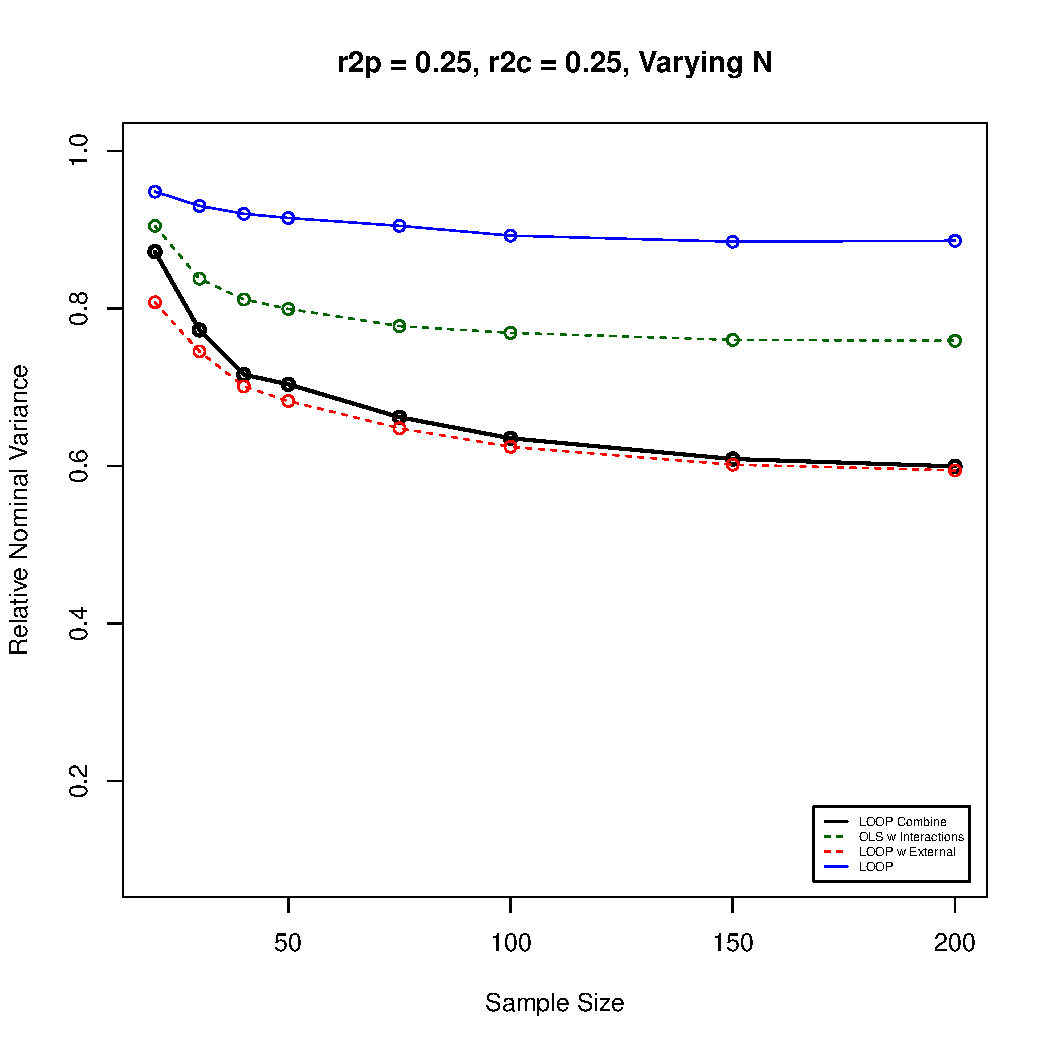
\includegraphics[width=.49\linewidth]{images/sampsize.pdf}
	\includegraphics[width=.49\linewidth,page = 2]{images/sampsize.pdf} \quad
	\smallskip
	\includegraphics[width=.49\linewidth,page = 3]{images/sampsize.pdf}
	\includegraphics[width=.49\linewidth,page = 4]{images/sampsize.pdf} \quad
	\caption{Top Left: $R^2_p = 0.25, R^2_c = 0.25$; Top Right: $R^2_p = 0.75, R^2_c = 0.25$; Bottom Left: $R^2_p = 0.25, R^2_c = 0.75$; Bottom Right: $R^2_p = 0.75, R^2_c = 0.75$}
\end{figure}
As we can see, when the predictive power is low for both the covariates and the external predictions ($R^2_p = 0.25, R^2_c = 0.25$), LOOP is outperformed by ReLOOP. Similarly, when the predictive power is high for both, ReLOOP outperforms LOOP. Even when $R^2_p$ is low and $R^2_c$ is high, the performance of ReLOOP quickly converges to the performance of LOOP. Finally we observe that ReLOOP does well at tracking the better performing component (and generally outperforms both components when the components perform similarly to each other).

\subsection{Varying Predictive Power of External Prediction}
For this simulation, we hold the predictive power of the covariates and sample size constant and vary $R^2_p = 0.05, 0.15, ..., 0.85, 0.95$. We consider four scenarios: (1) $N = 30, R^2_c = 0.25$; (2) $N = 30, R^2_c = 0.75$; (3) $N = 60, R^2_c = 0.25$; and (4) $N = 60, R^2_c = 0.75$:
\begin{figure}[H]
	\centering
	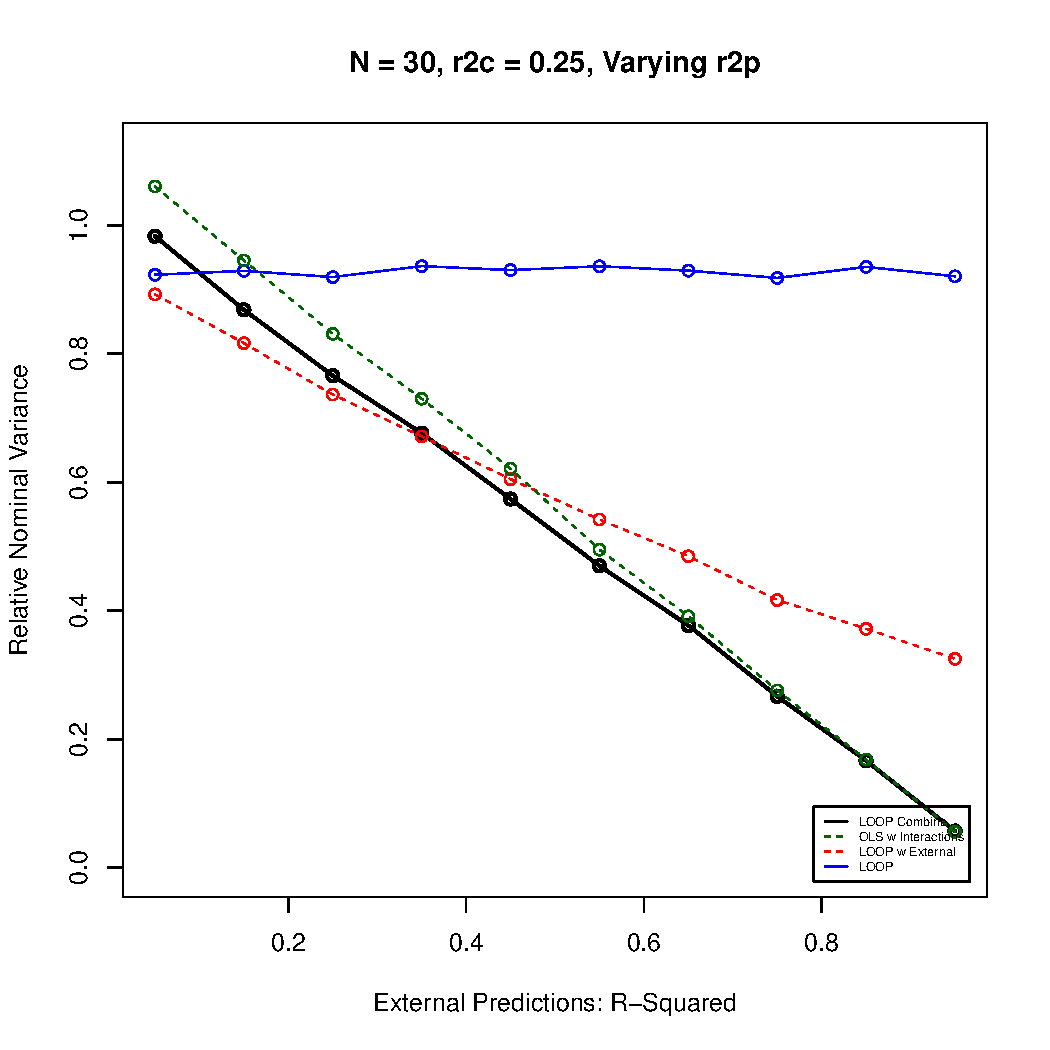
\includegraphics[width=.49\linewidth]{images/r2p.pdf}
	\includegraphics[width=.49\linewidth,page = 2]{images/r2p.pdf} \quad
	\smallskip
	\includegraphics[width=.49\linewidth,page = 3]{images/r2p.pdf}
	\includegraphics[width=.49\linewidth,page = 4]{images/r2p.pdf} \quad
	\caption{Top Left: $N = 30, R^2_c = 0.25$; Top Right: $N = 30, R^2_c = 0.75$; Bottom Left: $N = 60, R^2_c = 0.25$; Bottom Right: $N = 60, R^2_c = 0.75$}
\end{figure}
Once again, we observe that ReLOOP tends to perform at least as well as either component. This is particularly true for $N=60$, where ReLOOP closely follows (or drops below) the lower of the component lines. As expected, the three methods that incorporate the external predictions all improve as $R^2_p$ increases, while the performance of LOOP stays constant. We can see that ReLOOP is outperformed by LOOP when only when $R^2_p$ is much lower than $R^2_c$.

\subsection{Varying Predictive Power of Covariates}
For this simulation, we hold the predictive power of the external predictions and sample size constant and vary $R^2_c = 0.05, 0.15, ..., 0.85, 0.95$. We consider four scenarios: (1) $N = 30, R^2_p = 0.25$; (2) $N = 30, R^2_p = 0.75$; (3) $N = 60, R^2_p = 0.25$; and (4) $N = 60, R^2_p = 0.75$:
\begin{figure}[H]
	\centering
	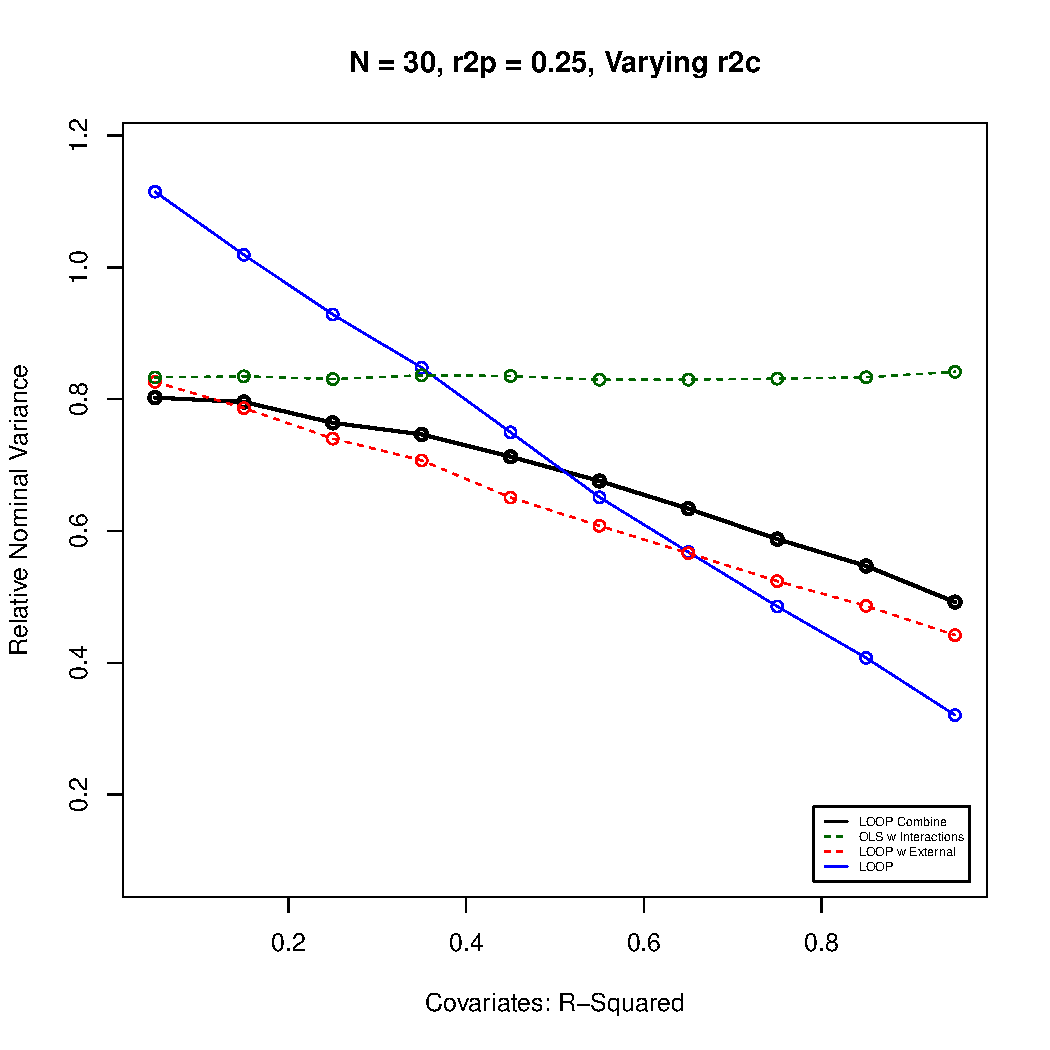
\includegraphics[width=.49\linewidth]{images/r2c.pdf}
	\includegraphics[width=.49\linewidth,page = 2]{images/r2c.pdf} \quad
	\smallskip
	\includegraphics[width=.49\linewidth,page = 3]{images/r2c.pdf}
	\includegraphics[width=.49\linewidth,page = 4]{images/r2c.pdf} \quad
	\caption{Top Left: $N = 30, R^2_p = 0.25$; Top Right $N = 30, R^2_p = 0.75$; Bottom Left $N = 60, R^2_p = 0.25$; Bottom Right: $N = 60, R^2_p = 0.75$}
\end{figure}
The performance of ReLOOP* stays constant, as the imputation method only incorporates the external predictions. The remaining methods all improve as $R^2_c$ increases. As before, we can see that ReLOOP tracks the better performing component well (especially when $N = 60$) and is only outperformed by LOOP when $R^2_c$ is much higher than $R^2_p$.

